% Chapter Template

\chapter{Network Components and Protocols} % Main chapter title

\label{Chapter3} % Change X to a consecutive number; for referencing this chapter elsewhere, use \ref{ChapterX}

\lhead{Chapter 3. \emph{Network Components and Protocols}} % Change X to a consecutive number; this is for the header on each page - perhaps a shortened title

%----------------------------------------------------------------------------------------
%	SECTION 1
%----------------------------------------------------------------------------------------
The purpose of this chapter is to present briefly the protocol or concepts that could be used throughout this paper.
\section{EAP}
The Extensible Authentication Protocol is a flexible authentication framework defined on the RFC3748 \cite{rfc3748}. EAP was designed to work without the IP protocol and provides support only for the transport of authentication protocols. The idea behind EAP was to creates a framework that supports several authentication methods and to separates the ahtentication methods from the transport.

\section{802.1X}
It's a IEEE standard that provides an authentication mechanism to devices on LAN or WLAN. Before explaining the standard, we will define the three parties involved.
\begin{itemize}
	\item[\texttt{Supplicant}] The client device that wants to connect to the network.
	\item[\texttt{Authentication Server}] The server that validates the credentials of the supplicants and determines the rights of the user.
	\item[\texttt{Authenticator}] A network device like a switch or an access point that is between the supplicant and the authentication server.
\end{itemize} 
802.1X is a port-based authentication protocol. Once a client connects to a publicly accessible port, the access control allows only the EAP traffic through that port. EAP is used to authenticate the supplicant and if the server grants the authorization to the supplicant, it can have access to the other services.
Each port have two state
\begin{itemize}
\item[Authorized] In this state, the supplicant is authenticated and have access to all its services.
\item[Unauthorized] The supplicant is not authorized and can only exchange EAP traffic with the authenticator.
\end{itemize}

\section{RADIUS}


\section{WiSM}



\section{DHCP}



\section{SNMP}

The Simple Network Management Protocol is an application layer protocol that facilitates the exchange of management information between network devices \cite{snmp}. It is part of the TCP/IP protocol suite and it is mainly used by network administrators to get information about devices on the network and the network performances. These information help the administrators to resolve problems on the network or simply to manage it.
A SNMP network has three main components:

\begin{itemize}
	\item \texttt{Network-management system (NMS)}: A NMS is the main component of an SNMP-managed network. It is the management entity that controls the managed devices. It uses the SNMP protocol and can interact with the managed devices to get information using special commands and messages.
	
	\item \texttt{Managed devices}: It is a network device that contains an SNMP agent. They collect and store information to make them available for the network-management systems. Those devices can be routers, servers, switches,etc. They also run the SNMP protocols to be able to respond to the requests made by the NMS.
	
	\item \texttt{Agents}: An agent is the thinking part of a managed device. It is a software module that understands the management information and translates them into a SNMP compatible form.
\end{itemize}

\begin{figure}[H]
\centering
	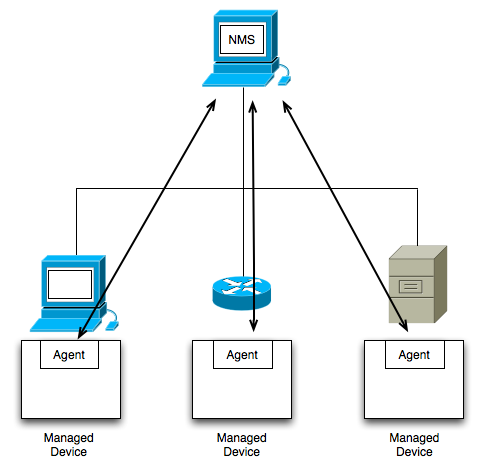
\includegraphics[width=.7\linewidth]{Pictures/Chapter3/snmp.png}
	\caption{A typical SNMP managed network}
\end{figure}

All the network objects are described and organized hierarchically in a Management Information Base (MIB). There are MIBs for each set of related network entites that can be managed. These MIBs are accessed using a network-management protocol such as SNMP.


\section{Problems encountered}